\chapter{Robust Record-Level Web Extraction Algorithm}
\label{ch:algorithm}
% Describe your own work (how you reached your goal) and take care to motivate your choices. Don't just describe all the things you did – tell us why.

In this chapter, we introduce our algorithm for a robust record-level data extraction. We explain the main concepts and describe the logic in detail.

Given an innitial web page snapshot with a single annotated book title, the algorithm extracts multiple movie titles from a future version of the same web page. The algorithm is designed to be fast and robust, require only a single annotated page for training, and extracts data from multiple records inside a tree.

To illustrate the principles, we use a deliberately simple example from Figure~\ref{fig:amazon-books-html} and extract book titles from a web page. The main steps are depicted in Figure~\ref{fig:algorithm}.

\begin{figure}[h]
	\centering
	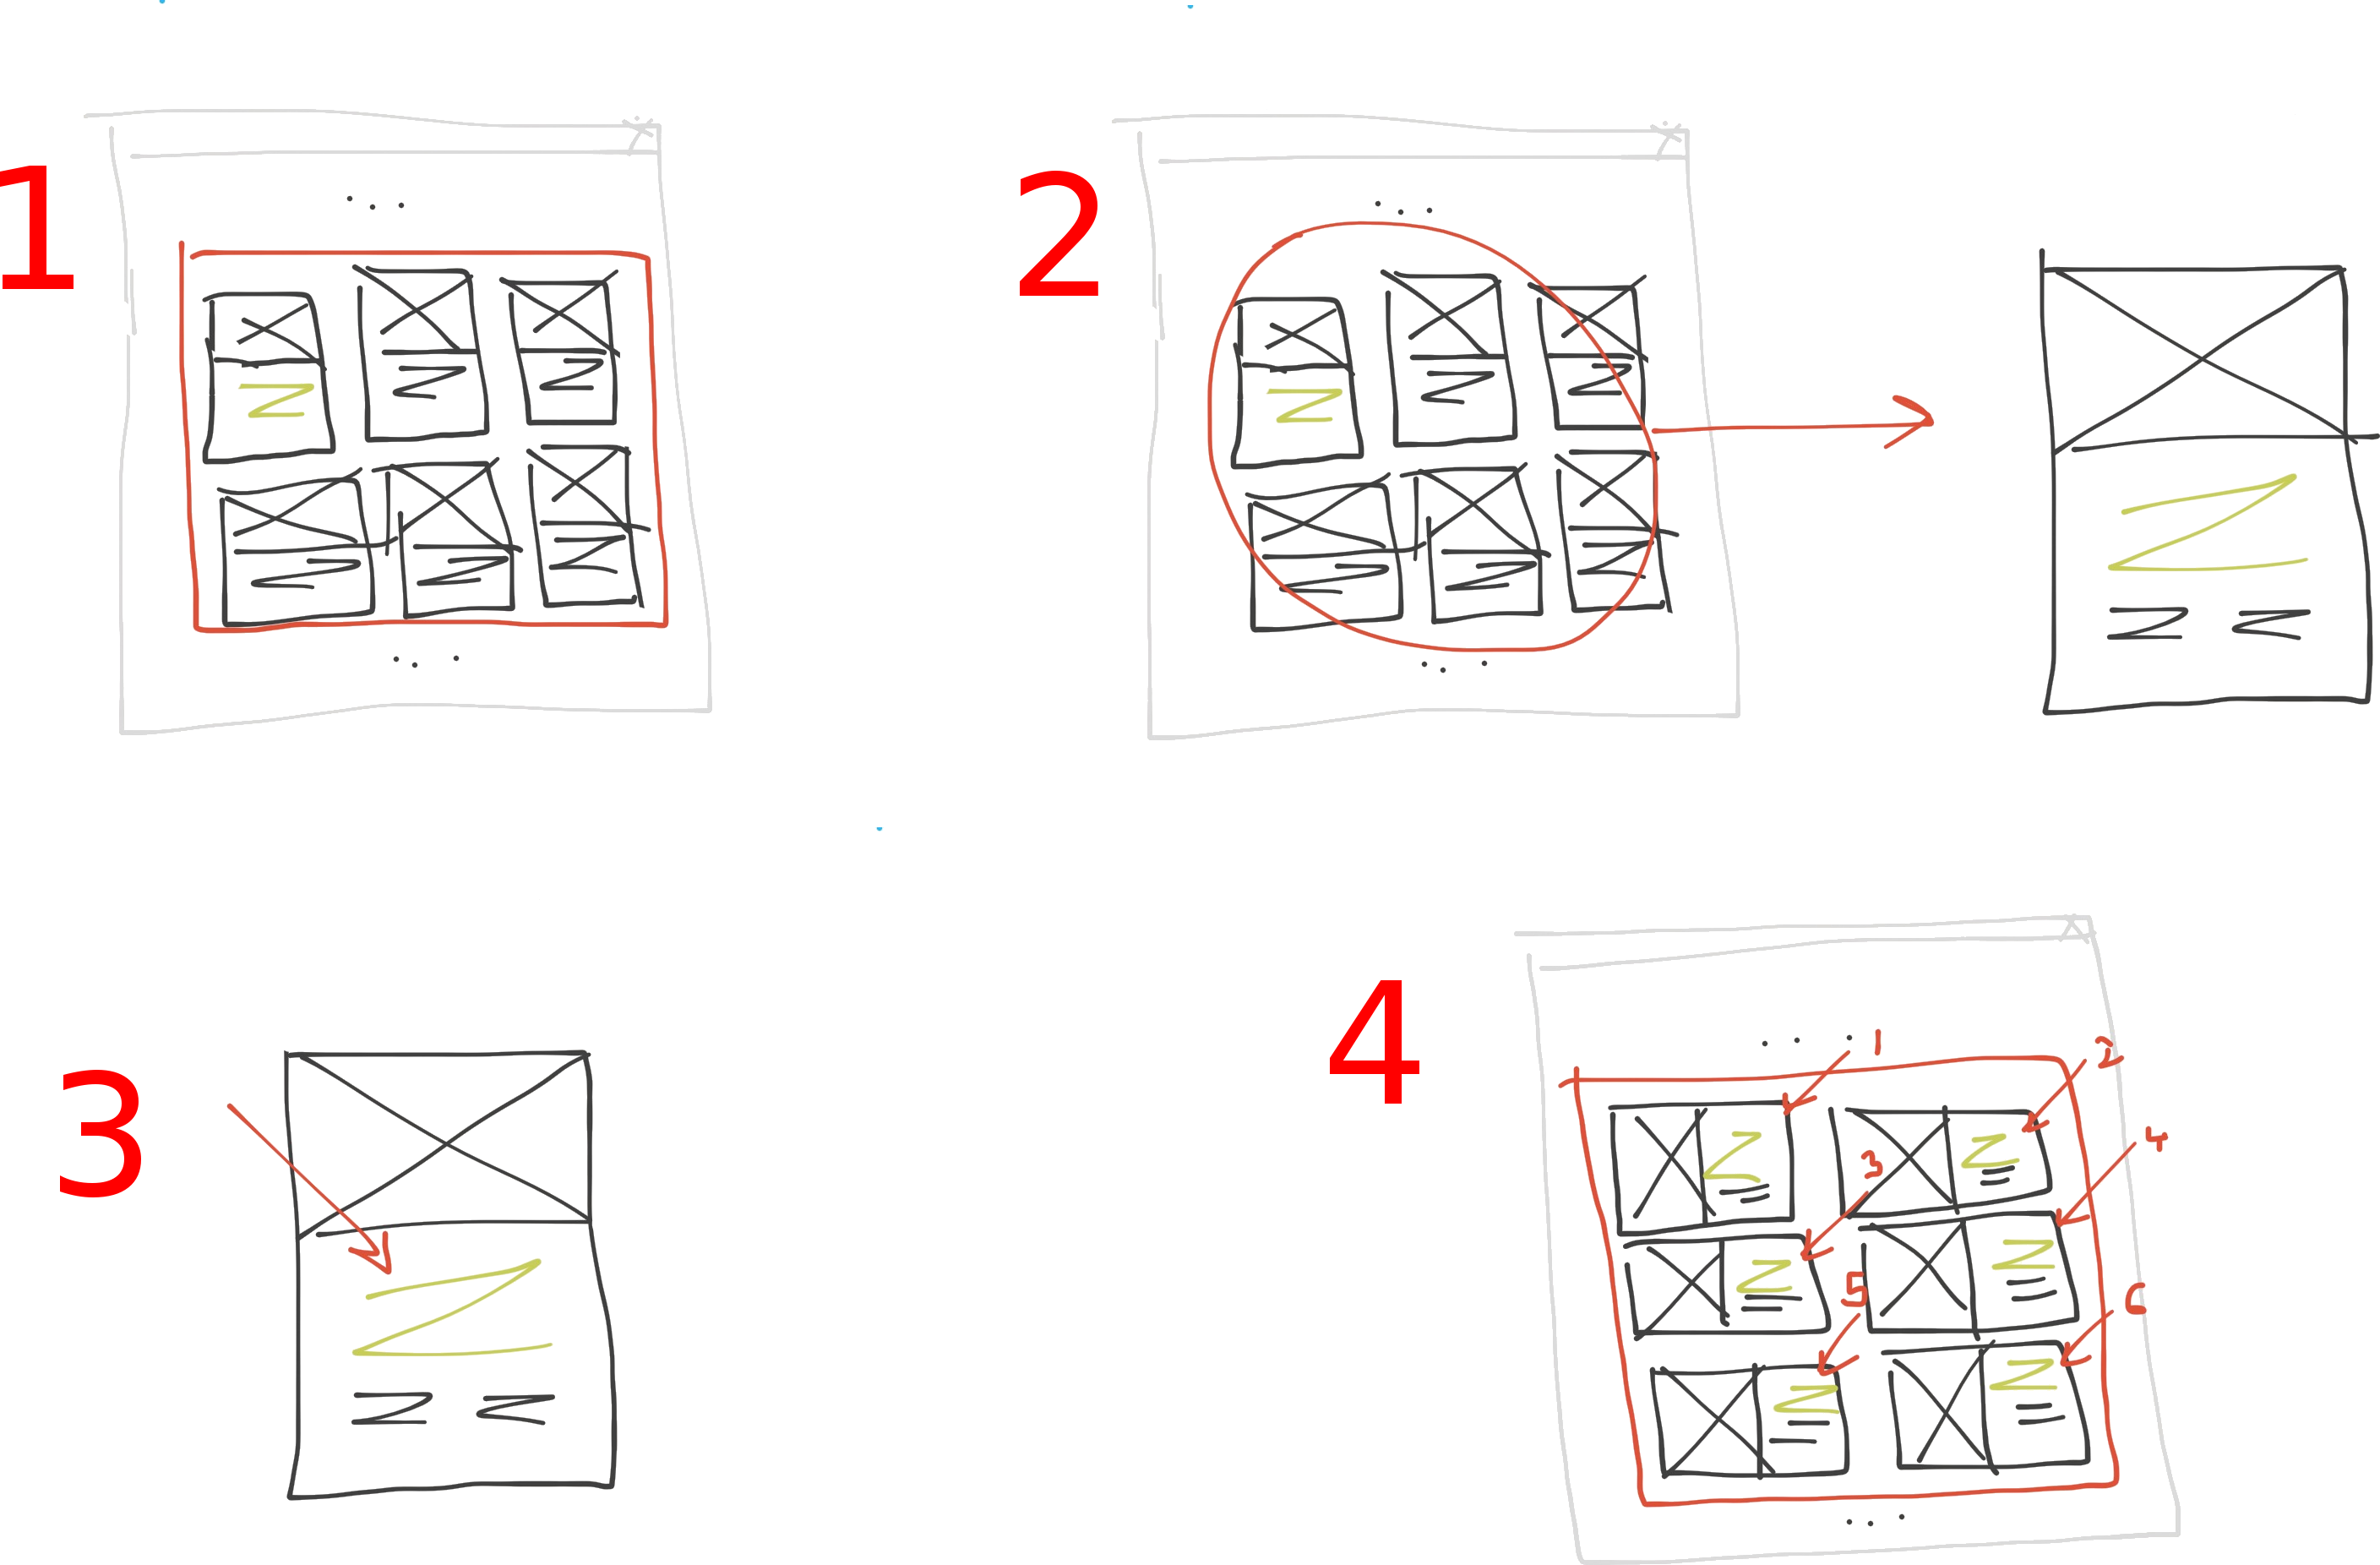
\includegraphics[width=1.0\textwidth]{figures/algorithm}
	\caption{Visualization of record-level wrapping steps.}
	\label{fig:algorithm}
\end{figure}

% How each method work. How they are combined.
The main idea of the new method is to split the wrapping process into two steps. First, we locate a relevant data region and find the boundaries of each data record. To cover structural variations, we progressively merge data records inside the original HTML into a generic tree. This tree is later used as an base for wrapping from the future pages. 

Next, we operate inside the boundary of each record in the transformed page and run a robust page-level wrapper. The wrapper is based on a tree-edit distance calculations with probabilistic HTML change model. The model captures how webpages evolve over time by looking at the likelihood of all possible changes \cite{dalvi2009a}.

% To illustrate the method in action..
[TODO] The following example illustrates sample inputs and outputs. An initial snapshot $w_{base}$ of a sample HTML document is illustrated in Figure~\ref{fig:sample-tree}. The annotated attribute node $d(w_{base})$ is marked with parenthesis. The extracted record attribute values are $\{\text{Carol}, \text{Bob}, \text{Alice}\}$.

% TODO step-by-step with given example

\begin{figure}[h]
	\centering
	\Tree [.table 
			[.tr 
				[.td [.img ] ]
				[.td 
					[.a
						[.\textit{How to Build...} ]
					]
					[.a
						[.\textit{George...} ]
					]
					[.span 
						[.\textit{Hardcover} ]
					]
					[. ... ]
				]
			]
			[.tr 
				[. ... ]
			]
		]
	\caption{An initial $w_{base}$ (on the left) and a transformed $w_{new}$ (on the right) snapshots of a sample HTML document. Distinguished nodes marked in paranthesis.}
	\label{fig:sample-tree}
\end{figure}

% TODO Consider a transformed tree from Fig.~xx



% ----------------------
\section{Core Algorithm}

% TODO inputs, outpus, introduce notation and definitions
A detailed method for robust record-level wrapping is given in Algorithm~\ref{alg:prob-record-level-wrapper}. It operates on labeled ordered rooted tree structures. Thus, this is not limited to HTML documents only. The algorithm extracts a set of candidate nodes from a transformed tree, given the initial tree with a distinguished node. The inputs and outputs of the algorithm are described below.

Inputs: 

\begin{enumerate}
	\item $w$ -- an initial (labeled ordered rooted) tree with embedded data records.
	\item $d(w)$ -- a distinguished node in the initial tree, i.e. a single attribute node of a random data record.
	\item $w'$ -- a transformed tree.
\end{enumerate}

Outputs: 

\begin{enumerate}
	\item $\{c'_i\}$ -- A set of extracted candate nodes in a transformed tree, i.e. single attribute values of all data records, e.g. book titles.
	%\item $c$ -- \emph{Confidence} measure, i.e. the probability measure that the wrapper did not break. This shows how accurate was the extraction.
\end{enumerate}

We assume that a distinguished node remains present in the future versions of the tree and is never deleted. The actual location of the node might change, though. For example, books listings web page in \url{amazon.com} will always contain book titles, even if the visual styling changes. This is a safe assumption, because the user annotates the tree by pointing out the content of interest. And this is typically an important piece of information, that is preserved over future (HTML document) updates. Thus, there is a single disinguished node $d(w) = \pi(d(w))$ in the new tree $w'=\pi(w)$, i.e. the node that a distinguished node $d(w)$ is mapped to by applying transformations $\pi$.

\IncMargin{2em}
\begin{algorithm}[h]

	\SetKwFunction{LocateDataRegionContainingNode}{LocateDataRegionContainingNode}
	\SetKwFunction{MergeDataRecords}{MergeDataRecords}
	\SetKwFunction{ProbWrap}{ProbWrap}
	\SetKwFunction{FindRegionContainingNode}{FindRegionContainingNode}
	\DontPrintSemicolon

	\KwData{$w, w', d(w)$}
	\KwResult{$\{c'_i\}$}
	\BlankLine

	$dr$ = \LocateDataRegionContainingNode($w$, $d(w)$) \;
	$r$ = \MergeDataRecords($dr$) \;

	$c'$ = \ProbWrap($w$, $d(w)$, $w'$) \;
	$dr'$ = \LocateDataRegionContainingNode($w'$, $c'$) \;

	\Return $\left\{ \ProbWrap(r, d(w), r') \right\}$, $\forall r' \in dr'$ \;

	\caption{Probabilistic record-level wrapper.}
	\label{alg:prob-record-level-wrapper}

\end{algorithm}
\DecMargin{2em}

% line-by-line how it works
The Algorithm~\ref{alg:prob-record-level-wrapper} first locates the data region $dr$ in the original tree $w$ that contains the distinguished node $d(w)$ as in Line 1. In Line 2, the data records from the data region $dr$ are merged into a generalized record $r$. As tree structure might slightly vary per record, this step ensures that the base record for wrapping contains the most general template. The candidate node $c'$ is identified on Line 3. With that, on Line 4 a data region $dr'$ in the trasnformed tree $w'$ is located. Finally, each data record $r'$ from the newly found data region $w'$ is locally wrapped with a probabilistic wrapper on Line 5.

% TODO Why it works?
% It would be nice if you could address correctness issues at some level. I would expect that proofs (formal or informal) would not be within reach, but you may add something like a discussion about what correctness means and how it can be addressed.


% The building blocks and motivation
The Algorithm~\ref{alg:prob-record-level-wrapper} consists of three main methods, which are described in the following sections:
\begin{description}
	\item[LocateDataRegionContainingNode] which recognizes template generated areas on a web page
	\item[MergeDataRecords] which generalizes records for multiple extraction
	\item[ProbWrap] which extracts data from a single data record in a robust way
\end{description}

% TODO What's the runtime? O(N)?
[TODO] The complexity of Algorithm~\ref{alg:prob-record-level-wrapper} is $O(n_1 k_1 n_2 k_2)$. The execution of \texttt{LocateDataRegionContainingNode} is the defining component as it has the complexity of $O(x)$.


% --------------------------------------------
\section{Locating Data Region Containing Node}

% Why? Alternatives? 
To enable wrapping in a web page with multiple data records, we need to locate individual data regions and run page-level wrapper inside a single region. Thus we chose \cite{liu2009a} proposed technique for data record mining. Unlike most alternatives [TODO: refs] this method supports both contiguous and non-contiguous data records, is more accurate than alternatives [TODO from Liu].

% TODO describe the limitation of the algo
As long as a page contains at least two data records, the algorithm will automatically find them.

% Inputs and outputs
Given a tree with embedded data records, the Algorithm~\ref{alg:locating-data-region-containing-node} locates a data region containing a distinguished node. The inputs / outputs are desribed in detail below.

Inputs: 

\begin{enumerate}
	\item $w$ -- a (labeled ordered rooted) tree with embedded data records.
	\item $v$ -- a distinguished node from a tree $w$.
\end{enumerate}

Outputs: 

\begin{enumerate}
	\item $dr$ -- a data record from a tree $w$ that contains a distinguished node $v$.
\end{enumerate}

% Reasoning behild the algo.
The algorithm is actually based on two observations. [BEGIN: dublicate] First, a group of data records have similar tree structure and are located in a close proximity. Second, these groups are under one parent node, i.e. it is very unlikely that a single record would begin inside one child subtree and end inside another child subtree. [END]


% TODO algo definition itself
\IncMargin{2em}
\begin{algorithm}[h]

	\SetKwFunction{TreeContainsNode}{TreeContainsNode}
	\SetKwFunction{MDR}{MDR}
	\SetKwFunction{Trees}{Trees}
	\DontPrintSemicolon

	\KwData{$w$, $v$}
	\KwResult{$dr$}
	\BlankLine

	$\left\{dr_i\right\}$ = \MDR($w$) \;
	\ForEach{$dr_i \in \left\{dr_i\right\}$} {
		\ForEach{$t_j \in \Trees(dr_i)$} {
			\If{\TreeContainsNode($t_j$, $v$)}{
				\Return $dr_i$ \;
			}
		}
	}

	\caption{Locating data region containing node}
	\label{alg:locating-data-region-containing-node}

\end{algorithm}
\DecMargin{2em}

% Step-by-Step
The detailed description of the method for locating a data region with a node is given in Algorithm~\ref{alg:locating-data-region-containing-node}. First, we locate all data regions per tree in Line 1. We make a call to Mining Data Records (MDR) algorithm as described in \cite{liu2009a}. This returns a set of all data regions found, not just the ones of interest. In lines 2-7 we iterate through all data regions and trees inside those regions, to locate the data record of interest. Finally, we return a data record with a node of interest.

% Original MDR shortcomings
In MDR, Liu et al. \cite{liu2009a} use string edit-distance for comparing child sub-trees. MDR traverses the tree from the root downward in a depth-first fashion. At each node, a  comparison of various combinations of the children sub-trees is performed. While this method is efficient (runtime complexity of $O(|s_1||s_2|)$, it is not accurate for text intensive web pages. As an example, consider two paragraphs with different text inside. String-wise these two are very different, yet the tree structure is identical (\texttt{<P>} element has a single child element \texttt{TEXT}).

% TODO: Zheng
- string edit distance is not suitable for this step as a string does not consider the tree structure, which is very useful in determining the correct alignment of data items.
- most tags used to form data records are tr’s and td’s. After string matching, it is hard to decide which alignment is the correct one as there are many possible alignments.
- tree matching significantly reduces the number of possible alignments because of the tree structure constraint.

% Updated MDR with tree edit-distance
Thus, we experimented with method variations by implementing tree-edit distance instead of original string edit-distance. We found the results to be more accurate. [TODO how?] But there was a penalty in execution time. Indeed, compared to string edit-distance, tree edit-distance runtime complexity is magnitude higher, i.e. $O(n^3)$. In this case, we decided to prioritize precision over the execution time. With further heuristics, the actual difference in execution time was not significant.

% Edit-tree distance: RTED
[TODO] Zheng'05
Several algorithms have been proposed to address the problem of
finding the minimum set of operations (i.e., the one with the
minimum cost) to transform one tree into another. All the
formulations have complexities above quadratic [10]. It has also
been shown that if the trees are not ordered, the problem is NP-
complete [36]. In [30], a solution based on dynamic programming
is presented. The algorithm has a complexity of O(n 1 n 2 h 1 h 2 ),
where n 1 and n 2 are the sizes of the trees and h 1 and h 2 are heights
of the trees. In [32][10], two other algorithms are also presented
with similar complexities.

[TODO] Pawlik and Augsten \cite{pawlik2011a} show that the efficiency of the previous solutions for the tree edit distance heavily depends on the tree shape and run into their worst cases for some data instances. They generalize the previous approaches and develop a new algorithm with O(n3) time (with n>m) and O(mn) space complexity. Their solution efficient for all tree shapes and never runs in the worst case if a better solution exists.

% Other params and optimizations
And also other optimiztions for our particular use-case: MAX-NUMBER-OF-TAGS-PER-GENERALIZED-NODE, EDIT-DISTANCE-THRESHOLD, areTableRows, substantiallyDifferentFrom

% Complexity analysis O(N)
$O(N K)$ plus the complexity of tree comparison which is $O(n^3)$


% ----------------------------
\section{Merging Data Records}

% Why? Alternatives?
Data records tend to have slight variations inside a data region. For example, in a book listing, certain books have special prices, while other don't. In order to reconstruct a full data record template structure, we progressively align multiple data record trees and merge them into a single template tree. TODO talk about alignment] [TODO refer to PartialTreeAlignment and Broom and WrapperGeneration] The idea of generalizing was mentioned in \cite{zheng2007a} and \cite{song2009a}.

% Inputs and outputs
Given a set of trees, the Algorithm~\ref{alg:merging-data-records} merges trees pairwise in a top-down order and returns a single merged template tree. Two trees are merged by subsequently aligning nodes layer-by-layer. If a node match is not found, then the algorithm attempts to expand the template tree by inserting the node into a template. The expanded template tree is then used in subsequent merging. Alignment takes into account only the structure of the tree, but not the data at the leaves. Input, output, and algorithm details are provided below.

Inputs: 

\begin{enumerate}
	\item $\left\{t_i\right\}$ -- a set of trees.
\end{enumerate}

Outputs: 

\begin{enumerate}
	\item $tt$ -- a merged template tree.
\end{enumerate}


\IncMargin{2em}
\begin{algorithm}[h]

	\SetKwFunction{SimpleTreeMatch}{SimpleTreeMatch}
	\SetKwFunction{AlignTrees}{AlignTrees}
	\SetKwFunction{FindUnalignedNodes}{FindUnalignedNodes}
	\SetKwFunction{InsertIntoSeed}{InsertIntoSeed}
	\DontPrintSemicolon

	\KwData{$\left\{t_i\right\}$}
	\KwResult{$tt$}
	\BlankLine

	$tt$ = $t_0$ \;
	\ForEach{$t \in \left\{t_i\right\}$}{
		$m$ = \SimpleTreeMatch($tt$, $t$) \;
		$l$ = \AlignTrees($m$) \;
		$u$ = \FindUnalignedNodes($t$, $l$) \;
		$tt$ = \InsertIntoSeed($tt$, $u$) \;
	}
	\Return $tt$ \;

	\caption{Merging data records}
	\label{alg:merging-data-records}

\end{algorithm}
\DecMargin{2em}

% step-by-step
Line 1 initializes the template with the first tree. Line 2 iterates through each tree to be merged and merges template with each tree pairwise. Line 3 evaluates similarity of two trees by producing the maximum matching matrix $m$ through dynamic programming. Line 4 aligns the nodes from the two trees by tracing back in the matrix $m$. Line 5 locates the unaligned vertexes $u$ from a tree $t$. These vertexes are inserted into a template in Line 6.

% what's different from Zhai
The Algorithm~\cite{alg:merging-data-records} is a variation of \emph{PartialTreeAlignment} by Zhai \cite{zhai2005a}. Methods \texttt{SimpleTreeMatch}, \texttt{FindUnalignedNodes}, \texttt{InsertIntoSeed} and \texttt{AlignTrees} are used from Zhai's work. An important distinction is the way these methods are composed. Unlike Zhai, we do not repeatedly try to match unaligned items with the template. We cannot allow any abiguity in the template, as it would impose undesired differences between template and data records in future wrapping. For example, adding unaligned node at a wrong position in the template would add additional edit cost of removing the node between two trees.

% Complexity analysis O(N)
[TODO]
In this method, a sequence x c that minimizes ($D(x_i, x_c)$ is the distance of two strings)
is selected as the center. Then a pair-wise alignment is performed
for each pair $(x_i, x_c)$, where $i != c$. Assuming there are $k$ sequences
and all sequences have length n, finding the center takes $O(k 2 n 2 )$
time and each step of the iterative pair-wise alignment takes $O(n 2 )$
time. Therefore the overall time cost is $O(k 2 n 2 )$.

[TODO Zheng 05] STM evaluates the similarity of two trees by producing the maximum matching through dynamic programming with complexity O(n 1 n 2 ), where n 1 and n 2 are the sizes of trees A and B respectively.


% ------------------------------
\section{Probabilistic Wrapping}

% Why? Alternatives? 
In the final step of the core Algorithm~\ref{alg:prob-record-level-wrapper}, a template tree is matched against new data records to locate the position of a distinguished node. We build on the work of Dalvi et al. \cite{dalvi2009a}, who formally define robustness, and Parameswaran et al. \cite{DBLP:journals/pvldb/ParameswaranDGR11}, who use HTML change model with tree edit-distance calculations to extract the data from a most probable location. Most alternative wrapping techniques [TODO: refs] require large training sets, or use no formal definition of robustness [TODO: refs], 
nd thus have weak confidence estimation.

% Inputs and outputs
Given an initial tree with a distinguished node, the Algorithm~\ref{alg:optimal-probabilistic-wrapper} locates the most probable candidate node in a transformed tree. This method calculates transformation probabilities for each candidate node and returns the one with the highest chance. The procedure precalculates probabilities for subtrees and thus later candidate iteration is not expensive.

Inputs: 

\begin{enumerate}
	\item $w$ -- an initial tree.
	\item $w'$ -- a transformed tree $w$.
	\item $u$ -- a distinguished node in initial tree $w$.
\end{enumerate}

Outputs: 

\begin{enumerate}
	\item $c$ -- the most probable location of a distinguished node $u$ in a transformed tree $w'$.
\end{enumerate}


\IncMargin{2em}
\begin{algorithm}

	\SetKwFunction{TP}{TP}
	\DontPrintSemicolon

	\KwData{$w, w', u$}
	\KwResult{$c$}
	\BlankLine

	\ForEach{$v \in w$}{
		$p_{1v}$ = \TP($P_1$, $P'_1$) \;
		$p_{2v}$ = \TP($P_2$, $P'_2$) \;
	}

	\ForEach{$t \subset w'$}{
		$p_{2v}$ = \TP($P_2$, $t$) \;
	}

	\ForEach{$v \in w'$}{
		\ForEach{$z \in P_2$}{
			$p_{2z}$ = \TP($P_{2v1z}$, $P'_{2v}$) \;
		}
		$p_{3v}$ = \TP($P_2$, $P'_2$) \;
		$Pr(v)$ = $p_{1v} \times p_{2v} \times p_{3v}$ \;
	}

	\Return $\operatorname*{arg\,max}_{v \in w} Pr(v)$ \;

	\caption{Optimal probabilistic wrapper.}
	\label{alg:optimal-probabilistic-wrapper}

\end{algorithm}
\DecMargin{2em}

In the description of Algorithm~\ref{alg:optimal-probabilistic-wrapper}, we use notation $T_v$ to note the tree under the node $v$, $P_1v$ to note all nodes in the tree that are to its left from node $v$ or to the left of its ancestors in some tree $w$, and $P_2$ to note the tree $w - T_v - P_1$.

% step-by-step
In the Algorithm~\ref{alg:optimal-probabilistic-wrapper}, the core function is $TP$, which calculates the probability of transforming one tree to another \cite{dalvi2009a}. It uses change model and tree-edit cost calculcations to perform the task. Lines 1-4 precalculcates probabilities of transforming prefix trees for all nodes. Lines 5-7 also precalcultes probabilities, but for transforming $P_2$ to complete subtrees in $w'$. Lines 9-11 precalcultes probabilities of prefix of $z$ in tree $P_2$ to tree $P'_2$. Final probability of transforming $P_2$ to $P'_2$ is calculated by Line 12. All of precalculated probabilities are multiplied in Line 13 to calculate the probability of $u$ being mapped to $v$. Finally, Line 15 returns the node $v$ with the highest probability.

% rewrite in own words
[TODO Talk about TP and its importance.]
TP calculates the probability of transforming a forest $f_1$ into a forest $f_2$, given insertion, deletion and substitution operations and their probabilities, i.e. change model. Implements function $DP_1(F_s, F_t)$, which calculates prob that $P_{\theta}(T|S)$, i.e. that $\pi(F_s) = F_t$.

\begin{equation}
	DP_1(F_s, F_t) = DP_2(F_s, F_t) + P_{ins}(v) \times DP_1(F_s, F_t - v)
\end{equation}

\begin{equation}
	\begin{split}
		DP_2(F_s, F_t) = P_{sub}(u, v) \times DP_1(F_2 - [u], F_t - [v]) \times DP_1(\lfloor u \rfloor, \lfloor v \rfloor) \\
		+ P_{del}(u) \times DP_2(F_s - u, F_t)
	\end{split}
\end{equation}



% Complexity analysis O(N)


% vim:wrap linebreak nolist:
